\begin{figure*}[t]
  \centering
  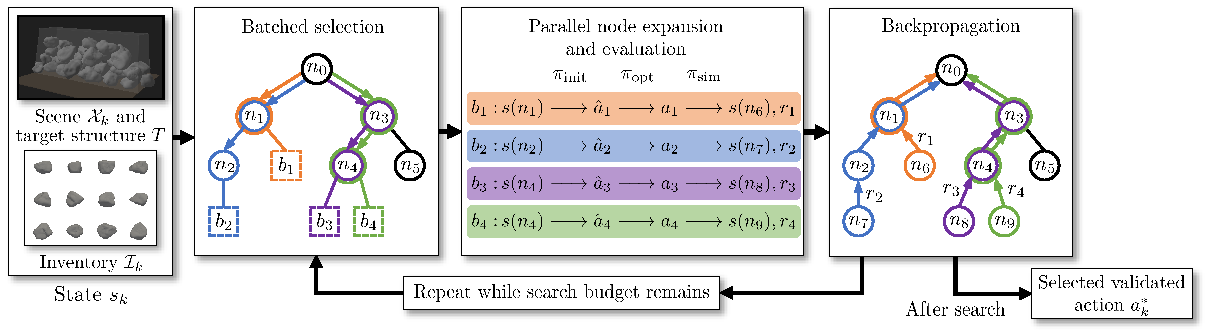
\includegraphics[width=0.94\textwidth]{figures/overview.pdf}
  \caption{Batched MCTS sequence planning. Colors identify expansion requests $b_j$ and their tree paths. Requests are evaluated in parallel through $\initpose$, $\poseopt$, and $\simul$, and returns are backpropagated along the selected paths. Search repeats within the budget before selecting a physically feasible root action $\action_k^*$ from the evaluated tree.}
  \label{fig:overview}
\end{figure*}


\section{Overview and Preliminaries} \label{sec:overview}

\subsection{Shape Representation}
We represent the target $\target$ and each object $\object_i$ as unions of smooth convex bodies modeled by differentiable support functions (DSFs)~\cite{lee2023uncertain}.
For a compact convex body $\convex\subset\real^3$, its support function is $\dsf_\convex(x)=\max_{p\in\convex}x^\top p$ for $x\ne0$.
At pose $q=(R,t)\in\SE(3)$, we write
\begin{equation*}
    \convex(q)=\{Rp+t\mid p\in\convex\},
    \qquad \object_i(q_i)=\bigcup_j\convex_{ij}(q_i),
\end{equation*}
where $\convex_{ij}$ are the convex components in object $i$'s local frame.
DSFs support differentiable signed-distance and contact-geometry computations between posed convex bodies~\cite{an2024riemannianmtd}, enabling gradient-based pose optimization.

\subsection{Markov Decision Process Formulation}

To address the construction objective in Eq.~\eqref{eq:problem_definition}, we model stacking as a finite-horizon sequential decision process in which one object is placed at each step. 
Let $\scene_k=\{(i,q_i)\mid i\in\placed_k\}$ be the current scene and $\inventory_k=\{1,\ldots,n\}\setminus\placed_k$ the remaining inventory. 
The state, action, and deterministic transition function are
\begin{equation*}
    \state_k=(\scene_k,\inventory_k,\target),\quad
    \action_k=(i_{k+1},q_{k+1}),\quad
    \state_{k+1}=\transition(\state_k,\action_k),
\end{equation*}
where $i_{k+1}\in\inventory_k$. The transition inserts the proposed pose into the scene, simulates the resulting structure, and returns the settled scene with $\inventory_{k+1}=\inventory_k\setminus\{i_{k+1}\}$. 
The reward $\reward(\state_k,\action_k)$ measures construction progress and physical validity; its implementation is described in Sec.~\ref{sec:sequence_planning}.
The sequence planner therefore operates on the MDP $\mdp=(\mathcal{S},\mathcal{A},\transition,\reward,\gamma)$.

\subsection{Monte Carlo Tree Search}

Monte Carlo Tree Search (MCTS) incrementally constructs a search tree $\tree=(\nodes,\edges)$ over the MDP. 
Each node $\node\in\nodes$ represents a state $\state(\node)\in\mathcal{S}$, and each edge $(\node,a)\in\edges$ represents an action $a\in\mathcal{A}$ and its transition to a child node. 
For a node or edge, let $\visit(\node)$ denote the number of completed evaluations and let $Q(\node)$ denote the empirical mean of the discounted returns backpropagated to that node. 
An action prior $P(\node,a)$, distinct from the transition function $\transition$, can provide additional guidance when the action space is large or continuous.

Each MCTS iteration consists of four conceptual operations. During \emph{selection}, the tree policy chooses a promising child by balancing its empirical value and an exploration bonus. 
During \emph{expansion}, a new action is generated and attached to the selected node. 
During \emph{evaluation}, the transition associated with the action is evaluated to obtain a reward and a successor state. 
Finally, during \emph{backpropagation}, the discounted return is propagated through the selected path to update $Q(\node)$ and $\visit(\node)$. 
A nonterminal leaf may additionally be assigned a leaf-value estimate $\hat V(\state)$, typically obtained from rollout simulation or a problem-specific heuristic.

In the present problem, an action is a placement of one remaining object, and its evaluation includes pose refinement and physical simulation. 
The geometry-informed proposals, batched selection, and finite-horizon leaf evaluation used to adapt MCTS to this expensive continuous-action setting are described in Sec.~\ref{sec:sequence_planning}.

\subsection{Overall Structure of the Sequence Planner}

The overall structure of the sequence planner is illustrated in Fig. \ref{fig:overview}. 
The sequence planner uses Monte Carlo Tree Search (MCTS) to explore the space of possible stacking sequences. 
For each expansion, the initial pose sampler $\initpose$ proposes a candidate action $\hat{\action}_k=(i_{k+1},\hat{q}_{k+1})$, specifying both the object index and its initial pose.
The pose optimization module $\poseopt$ refines the pose component to obtain $\action_k=(i_{k+1},q_{k+1})$.
The structural simulation module $\simul$ subsequently implements the physical transition by evaluating the entire provisional scene and producing the settled next state. 
The resulting validity and simulation statistics are used to determine whether the action is admitted to the search tree and to evaluate its reward.

This gives the following execution flow:
\begin{equation*}
\state_k
\xrightarrow{\ \initpose\ }
\hat{\action}_k
\xrightarrow{\ \poseopt\ }
\action_k
\xrightarrow{\ \simul\ }
\state_{k+1},\ \reward(\state_k,\action_k).
\end{equation*}
We describe pose optimization in Sec. \ref{sec:pose_optimization} and sequence planning, including structural simulation and reward design, in Sec. \ref{sec:sequence_planning}.
